\documentclass[11pt]{article}
\usepackage{nodalida2017}
%\usepackage{times}
\usepackage{mathptmx}
%\usepackage{txfonts}
\usepackage{xcolor}
\usepackage{graphicx}
\usepackage{url}
\usepackage{latexsym}
\usepackage{listings}
\special{papersize=210mm,297mm} 


\title{Exploring the Expressivity of Constraint Grammar}

% \author{First Author \\
%   Affiliation / Address line 1 \\
%   {\tt email@domain} \\\And
%   Second Author \\
%   Affiliation / Address line 1 \\
%   {\tt email@domain} }

\date{\today}

\def\t#1{\texttt{#1}}
\def\h#1{{\tt \color{gray} #1}}
\def\swf{\h{"<s>"}}
\def\maxAmb#1{$\langle \Sigma \rangle_#1$}
\def\maxAmbFSA#1{$\langle \Sigma,S \rangle_#1$}
\def\maxAmbCFG#1{$\langle \Sigma,\Sigma^{\prime} \rangle_#1$}

\begin{document}
\maketitle

\begin{abstract}
  We believe that for any formalism which has its roots in linguistics, it is a
  natural question to ask ``how expressive is it?'' Therefore, in this paper, we
  begin to address the question of the expressivity of CG.
  Aside from the obvious theoretical interest, we envision also practical
  benefits. For instance, we hope that the \texttt{cgexp} tool, described in
  later sections of this paper, could eventually be developed to generate
  human-readable CG code from regular expressions or a context-free grammar. 
\end{abstract}

\section{Introduction and previous work}

CG~\cite{karlsson1995constraint} was born as a practical, rather than formal, 
approach to NLP. 
Since the beginning, its authors do not envision it as a tool for 
generating strings, only for analysing and disambiguating them.
It is for these reasons, we believe, that the question of the expressivity of CG
as a generative formalism went unasked and unanswered for so long.

The standard measure of formal languages is the Chomsky
hierarchy~\cite{chomsky1956hierarchy}, with its four classes of grammars and
languages, in order from most expressive to least expressive: recursively
enumerable (Type 0), context-sensitive (Type 1), context-free (Type 2), and
regular (Type 3). The notion of expressive power, ``which constructs can we
express in the language'', is coupled with parsing complexity, ``how much time
and memory do we need to parse sentences in the language''; more expressive
power corresponds to greater parsing complexity.


%Previous work covers the expressivity of single rules,
%such as \texttt{IF (NOT 1* Verb OR Noun)}: just seeing this contextual test hints that we can express
%a subset of regular languages that contains at least disjunction, complement and Kleene star. 
\newcite{tapanainen1999phd} gives an account of the expressivity of
the contextual tests for 4 different constraint formalisms, including CG. 
In addition, parsing complexity can be easily defined for a given variant and 
implementation of CG; see for instance \newcite{nemeskey14}.
However, to our knowledge, expressivity of a whole grammar has not been approached before.

In the following section, we discuss our approach to CG as a formal language.
Then, in the remainder or this paper, we discuss a number of preliminary
results.

\section{Expressivity of a constraint grammar}

For this paper, we will view a constraint grammar CG as generating a formal
language $\mathcal{L}$ over an alphabet $\Sigma$ as follows:
A constraint grammar CG rejects a word $w \in \Sigma^\star$ if, when we encode
the word as a sequence of cohorts, and pass it through the CG, we get back the
dedicated rejection cohort \texttt{<REJECT>}. A constraint grammar CG accepts a
word $w \in \Sigma^\star$ if it does not reject it. 

As an example, consider the language $a*$ over $\Sigma = \{a,b\}$. This language
can be encoded as a constraint grammar as in Figure~\ref{fig:astar}. We then
encode the input as cohorts (e.g.\ \t{"<a>"}, \t{"<b>"}), and run the grammar.
See Figure~\ref{fig:astario} for two example runs.

\begin{figure}[h]
  \begin{verbatim}
    LIST A = "<a>";
    LIST B = "<b>";
    SET LETTER = A OR B;
    ADDCOHORT ("<REJECT>")
      BEFORE LETTER 
      IF (-1 (>>>) LINK 1* B);
    REMCOHORT LETTER
      IF (-1* ("<REJECT>"));
  \end{verbatim}
  \caption{A constraint grammar which generates the language $a^\star$.}
  \label{fig:astar}
\end{figure}

\begin{figure}[h]
  \centering
  \begin{tabular}{c|c}
    \textbf{Input} & \textbf{Output} \\ \hline
    \t{"<a>"}      & \t{"<REJECT>"} \\
    \t{"<a>"}      \\
    \t{"<b>"}      \\ \hline
    \t{"<a>"}      & \t{"<a>"} \\
    \t{"<a>"}      & \t{"<a>"} \\
    \t{"<a>"}      & \t{"<a>"}
  \end{tabular}
  \caption{Examples of input and output for the grammar in
    Figure~\ref{fig:astar}.}  
  \label{fig:astario}
\end{figure}


\section{A lower bound for CG}

It should be noted that VISL CG-3 \cite{bick2015,vislcg3} supports commands 
such as \t{EXTERNAL}, which runs an external executable. It should therefore 
be obvious that the complete set of CG-3 commands, at least theoretically, 
can generate any recursively enumerable language. For this reason, we restrict 
ourselves to a subset of the commands permitted by CG.

In this section, we will only use the \t{REMOVE} command with sections, in
addition to a single use of the \t{ADDCOHORT} command to add the special cohort
\t{"<REJECT>"}, and a single use of the \t{REMCOHORT} command to clean up
afterwards. 
We show that, using only these commands, CG is capable of generating some
context-free and context-sensitive languages, which establishes a lower bound on 
the expressivity of CG (see Figure~\ref{fig:nocorr}).

\begin{figure}[h]
  \centering
  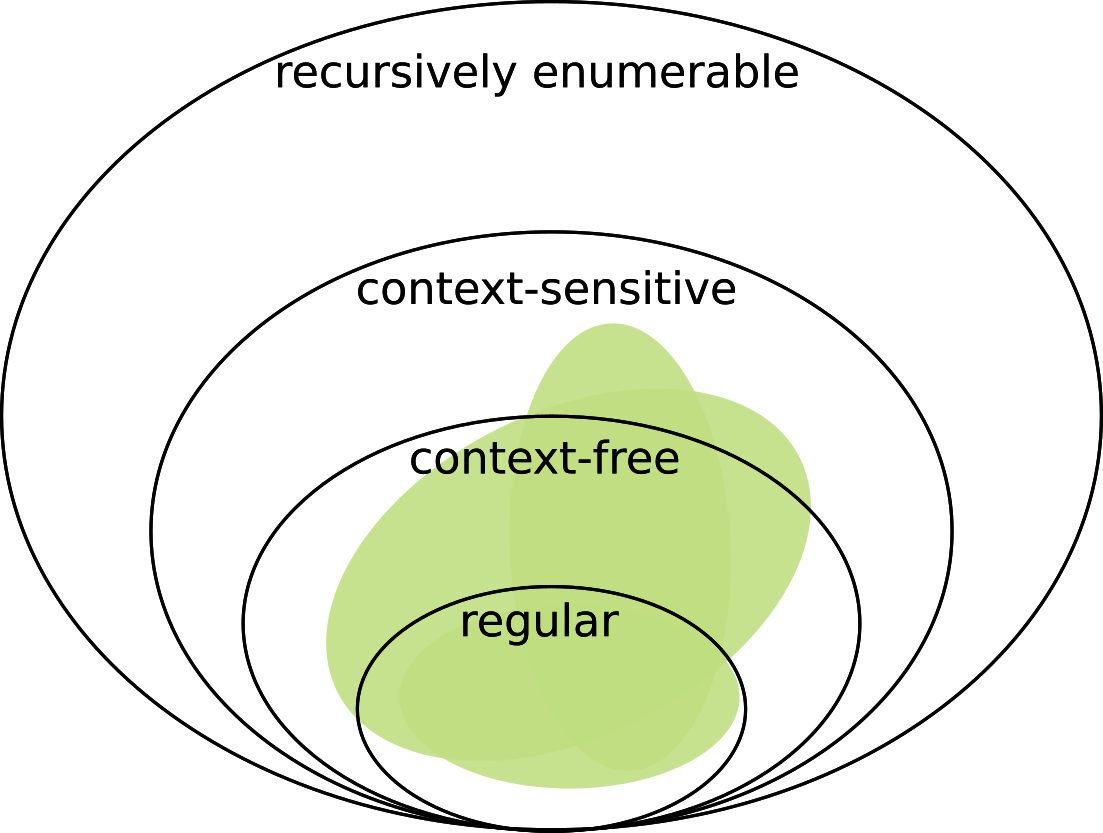
\includegraphics[width=0.8\linewidth]{chomsky}
  \caption{Lower bound on the expressivity of CG.}
  \label{fig:nocorr}
\end{figure}

\subsection{Example grammar: $a^nb^n$ }

Below, we briefly describe the CG which generates the language $a^nb^n$.
This CG is defined over the alphabet $\Sigma$, in addition to a hidden alphabet
$\Sigma^\prime$. These hidden symbols are meant to serve as a simple form of
memory. When we encode our input words, we tag each cohort with \emph{every}
symbol in the hidden alphabet\footnote{
  This can be implemented in CG using the \t{ADD} command.
  Our approach, however, is more restricted. 
} (e.g. \t{"<letter>" hidden$_1$} \dots \t{hidden$_n$}).

This CG uses the hidden alphabet \{\t{odd}, \t{even}, 
% \t{>>>}, \t{<<<}\footnote{
%   These \emph{can} be the magic begin and end tags provided by CG, however, they
%   can also be implemented using two hidden symbols and the \t{REMOVE} command.
%   Therefore, whichever is chosen does not matter for the expressivity.
% }, 
\t{opt\_a}, \t{opt\_b}\}.
These symbols mean that the cohort they are attached to is in an even or odd
position, 
% in first or last position, 
and that $a$ or $b$ is a legal option for this cohort, respectively. 
The CG operates as follows:
\begin{enumerate}
\item
  Is the number of characters even? We know the first cohort is odd, and the
  rest is handled with rules of the form \t{REMOVE even IF (NOT -1 odd)}. If the
  last cohort is odd, then discard the sentence. Otherwise continue\dots
\item
  The first cohort is certainly $a$ and last is certainly $b$, so we can
  disambiguate the edges: 
  % \t{REMOVE opt\_b IF (0 >>>)}, and \t{REMOVE opt\_a IF (0 <<<)}. 
  \t{REMOVE opt\_b IF (NOT -1 (*))}, and \t{REMOVE opt\_a IF (NOT 1 (*))}. 
\item
  Disambiguate the second cohort as $a$ and second-to-last as $b$, the third as
  $a$ and third-to-last as $b$, etc, until the two ends meet in the middle. If
  every \t{"<a>"} is marked with \t{opt\_a}, and every \t{"<b>"} with
  \t{opt\_b}, we accept. Otherwise, we reject.  
\end{enumerate}
The language $a^nb^n$ is context-free, and therefore CG must at least partly
overlap with the context-free languages.

\subsection{Example grammar: $a^nb^nc^n$}

We can extend the approach used in the previous grammar to write a grammar which
accepts $a^nb^nc^n$. Essentially, we can adapt the above grammar to find the
middle of any input string. Once we have the middle, we can ``grow'' $a$s from
the top and $b$s up from the middle, and $b$s down from the middle and $c$s up
from the bottom, until we divide the input into three even chunks.
If this ends with all \t{"<a>"}s marked with \t{opt\_a}, all \t{"<b>"}s marked
with \t{opt\_b}, and all \t{"<c>"}s marked with \t{opt\_c}, we accept.
Otherwise, we reject.

The language $a^nb^nc^n$ is context-sensitive, and therefore CG must at least
partly overlap with the context-sensitive languages. 


\section{Are all regular languages in CG?}

Is CG in any particular category? It clearly covers some regular, context-free
and context-sensitive languages, but it may just have a common subset with those 
classes, as in Figure~\ref{fig:nocorr}.
Rather than enumerating individual grammars for a given class, we need a method 
that can transform all languages in that class into CG.


We present a method to transform arbitrary finite-state automata into CG.\footnote{A subset which includes \t{LINK}, \t{NEGATE} and \t{TEMPLATE}, in addition to the previous.}
Figure~\ref{fig:fsa} presents an example automaton with $\Sigma = \{$\emph{det, adj, n}$\}$,
for which we implement a corresponding CG as follows.

As previously, we define a hidden alphabet $\Sigma^{\prime} = \{$\t{opt\_det, opt\_adj, opt\_n}$\}$,
and insert the full set to each cohort. 
In addition, we introduce \emph{state cohorts}, which contain the full set $S = \{s_1, s_2\}$.
For example, the sequence \emph{det n} would be modelled with the following sentence:

\begin{table}[h]
\begin{tabular}{c|c|c|c|c}
   \swf   &   \t{"<det>"}  &  \swf      &   \t{"<n>"} &  \swf     \\ \hline
 \h{s1}   & \t{opt\_det}   &  \h{ s1}   &  \t{opt\_det}  &  \h{s1}  \\
 \h{s2}   & \t{opt\_adj}   &  \h{ s2}   &  \t{opt\_adj}  &  \h{s2}  \\
          & \t{opt\_n}  &            &  \t{opt\_n} &  
\end{tabular}
\end{table}

The rules of the grammar disambiguate both word cohorts and state cohorts.
Thus the desired result shows both the accepted string and the path in the automaton.

\begin{table}[h]
\centering
\begin{tabular}{c|c|c|c|c}
   \swf   &   \t{"<det>"}  &  \swf   & \t{"<n>"}    &  \swf     \\ \hline
  \h{s1}  & \t{opt\_det} &  \h{s2}   &  \t{opt\_n}  &  \h{s1} 

\end{tabular}
\end{table}



\begin{figure}[t]
  \centering
    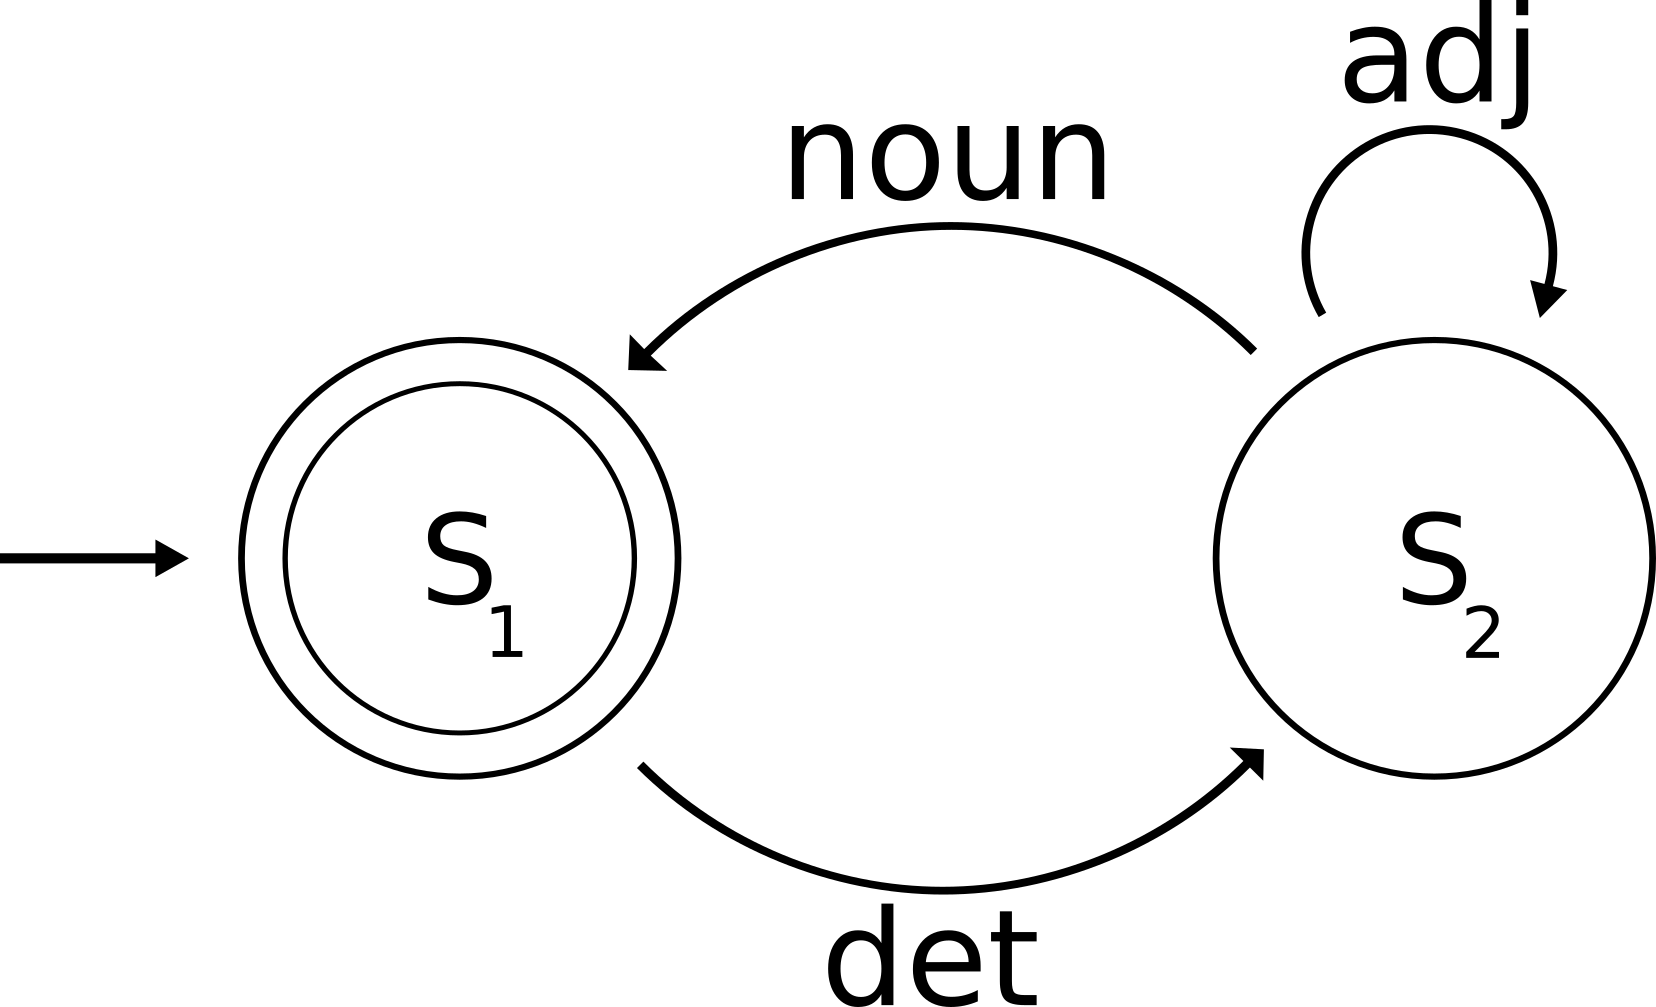
\includegraphics[width=0.7\linewidth]{fsa.png}
  \caption{A finite-state automaton describing the regular language \t{det (adj)* n}.}
 \label{fig:fsa}
\end{figure}


\subsection{Disambiguation process}

% We describe the process on a high level. We have a working implementation that
% produces the rules for arbitrary automata, but the following is by no means a formal proof.

Given that every transition happens between two states, and every state 
has an incoming and outgoing transition, every rule needs no more than
positions -1 and 1 in their contextual tests. 
The semantics of the rules are ``remove a POS tag, if it is \emph{not} surrounded by allowed states'',
and ``remove a state, if it is \emph{not} surrounded by allowed transitions''.
For the example automaton, the POS-rules are as follows.

\begin{verbatim}
REMOVE...
   OptDet IF (NEGATE -1 S1 LINK 2 S2) ;
   OptAdj IF (NEGATE -1 S2 LINK 2 S2) ;
   OptN   IF (NEGATE -1 S2 LINK 2 S1) ;
\end{verbatim}

The start and end states naturally correspond to the first and last state cohort 
in the \maxAmbFSA{n}, and can be trivially disambiguated, in this case both into \t{s1}.
Once we remove a reading from either side of a cohort, some more rules 
can take action---the context ``\t{s2} on the left side and \t{s1} on the right side''
may be broken by removing either \t{s2} or \t{s1}.
As a chain reaction, the whole sentence gets eventually disambiguated.

\subsection{Disjunction}

Consider the regular language with two strings $\{ab,ba\}$. 
Given \maxAmb{2} for any $\Sigma$, this is the closest we could get in CG output:

\begin{table}[h]
\begin{tabular}{r|r}

  \t{"<a>"}    &    \t{"<b>"}  \\ \hline
   \t{opt\_a}  &  \t{opt\_a}  \\
   \t{opt\_b}  &  \t{opt\_b}
\end{tabular}
\end{table}

As \newcite{lager_nivre01} point out, CG has no way of expressing disjunction.
Unlike its close cousin FSIG \cite{koskenniemi90}, which would represent this language
faithfully, CG substitutes uncertainty on the sentence level (``either $ab$ or $ba$'')
with uncertainty in the cohorts:
``the first character may be either $a$ or $b$, and the second character may be either $a$ or $b$''.

An alternative would be to model languages with disjunction as a set of CGs: 
one that disambiguates any input into $ab$ and other that disambiguates 
into $ba$. But this is just speculation, we have not investigated the idea further. 

% The start and end states naturally correspond to the first and last state cohort 
% in the \maxAmbFSA{n}, and can be trivially disambiguated, in this case both into \t{s1}.
% The intermediate result is shown below:

% \def\rmd#1{{\tt \color{gray} #1}}

% \begin{table}[h]
% \centering
% \begin{tabular}{lllll}
%      \swf &  \wwf   &      \swf &     \wwf &     \swf \\
% ~~~~~~\t{s1}   & ~~~~\t{det}  &  ~~~~\t{s1}   &  ~~~~\t{det}  &  ~~~~\t{s1}   \\
% ~~~~~~\rmd{s2} & ~~~~\t{adj}  &  ~~~~\t{s2}   &  ~~~~\t{adj}  &  ~~~~\rmd{s2}   \\
% ~~~~~~         & ~~~~\t{noun} &                &  ~~~~\t{noun} &  
% \end{tabular}
% \end{table}

% Once we remove a reading from either side of a cohort, some more rules may take action.
% Now that the first state is no longer a possible \t{s2}, the rules that remove \t{adj}
% and \t{noun} readings will apply to the first word.

% \begin{table}[h]
% \centering
% \begin{tabular}{lllll}
%      \swf &  \wwf     &      \swf &     \wwf &     \swf \\
% ~~~~~~\t{s1}   & ~~~~\t{det}    &  ~~~~\t{ s1}   &  ~~~~\t{det}  &  ~~~~\t{s1}   \\
% ~~~~~~\rmd{s2} & ~~~~\rmd{adj}  &  ~~~~\t{ s2}   &  ~~~~\t{adj}  &  ~~~~\rmd{s2}   \\
% ~~~~~~         & ~~~~\rmd{noun} &                &  ~~~~\t{noun} &  
% \end{tabular}
% \end{table}

% Now the second state cohort can be disambiguated: transitions from \t{det} may only lead to \t{s2}, 
% so we remove \t{s1}. After that, we disambiguate the second word cohort, leaving only \t{noun}.
% No more rules may apply, so this is the final result.

% \begin{table}[h]
% \centering
% \begin{tabular}{lllll}
%       \swf &  \wwf     &      \swf &     \wwf  &     \swf \\
%  ~~~~~~\t{s1}   & ~~~~\t{det}    &  ~~~~\rmd{s1}  &  ~~~~\rmd{det} &  ~~~~\t{s1}   \\
%  ~~~~~~\rmd{s2} & ~~~~\rmd{adj}  &  ~~~~\t{s2}    &  ~~~~\rmd{adj} &  ~~~~\rmd{s2}   \\
%  ~~~~~~         & ~~~~\rmd{noun} &                &  ~~~~\t{noun}  &  
% \end{tabular}
% \end{table}




\section{Applications}

Does such an idea provide any foreseeable practical benefits?
The grammars derived from FSAs look clumsy, and involve extra symbols.
But if it turned out that CGs can express some interesting subset of context-free 
or context-sensitive grammars, then we could derive CGs from already existing formalisms.
This could be an alternative for learning CGs from corpus.

Compared to high-level grammar formalisms, such as (insert your favourite), CG processing
is generally faster. So a CG derived in this manner could act as a preprocessing step 
for some more expensive parser---then the rules need not be human-legible. 
The rules would be derived from the grammar itself, with the sole purpose of 
making the parsing \emph{faster}, not more accurate.



% \section*{Acknowledgments}

% Do not number the acknowledgment section. Do not include this section
% when submitting your paper for review.





\bibliographystyle{acl}
\bibliography{cg}


\end{document}
